\chapter{Dob�r parametru $\lambda$}

Dla rozmytego algorytmu DMC z zadania 6 b�dziemy teraz kalibrowa� wsp�czynnik lambda, tak aby otrzyma� jak najlepsz� jako�� regulacji na ca�ym przebiegu. Dob�r tych parametr�w b�dzie za pomoc� metody in�ynierskiej, czyli metod� iteracyjn�, poniewa� dob�r tych parametr�w wymaga wiele pr�b to poni�ej zamie�cimy tylko wyniki kalibracji.



%\begin{center}
%\begin{figure}[H]
%\makebox[\textwidth]{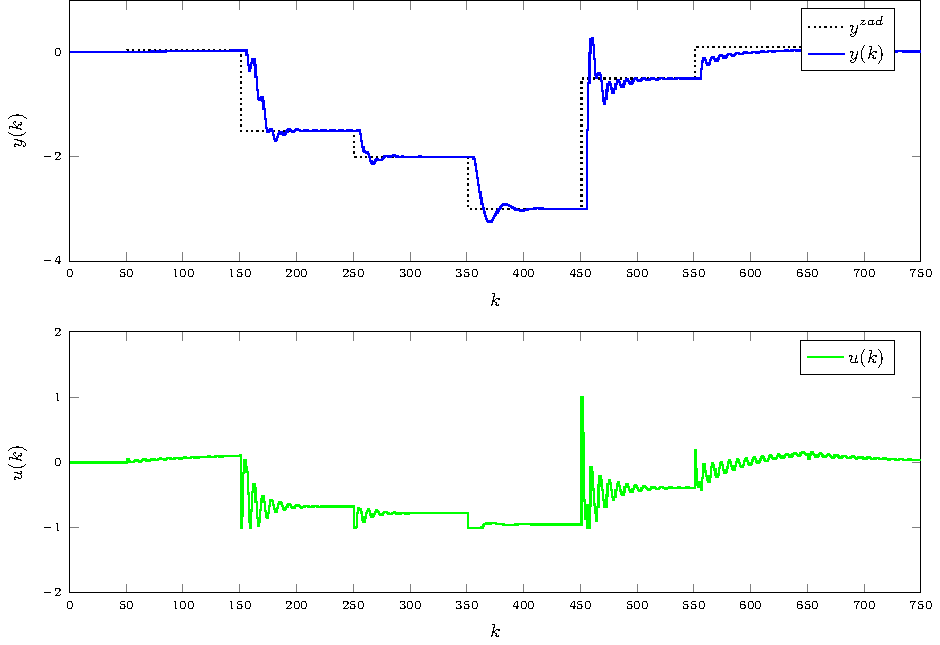
\includegraphics[width=\paperwidth]{data/exercise_7/Desired_plot_DMC_number_of_fuzzy_reg_1.pdf}}
%\label{Desired_plot_DMC_number_of_fuzzy_reg_1}
%\caption{eg=1}
%\end{figure}
%\end{center}

\begin{table}[H]
\centering
\begin{tabular}{ | m{5em} | m{5em} |m{5em} |m{5em} |m{5em} |m{5em} | }
\hline
$D$ & $N$ & $N_u$ & $\lambda$ & $c$ & $\sigma$ \\
\hline
$\num{25}$ & $\num{15}$ & $\num{10}$ & $\num{0.1}$ & $\num{-2.5}$ & $\num{0.6}$\\
\hline
$\num{25}$ & $\num{15}$ & $\num{10}$ & $\num{0.1}$ & $\num{-0.7}$ & $\num{0.6}$\\
\hline
\end{tabular}
\label{eksperyment2_DMC}
\caption{Parametry 2 rozmyte regulatory DMC}
\end{table}

\begin{center}
\begin{figure}[H]
\makebox[\textwidth]{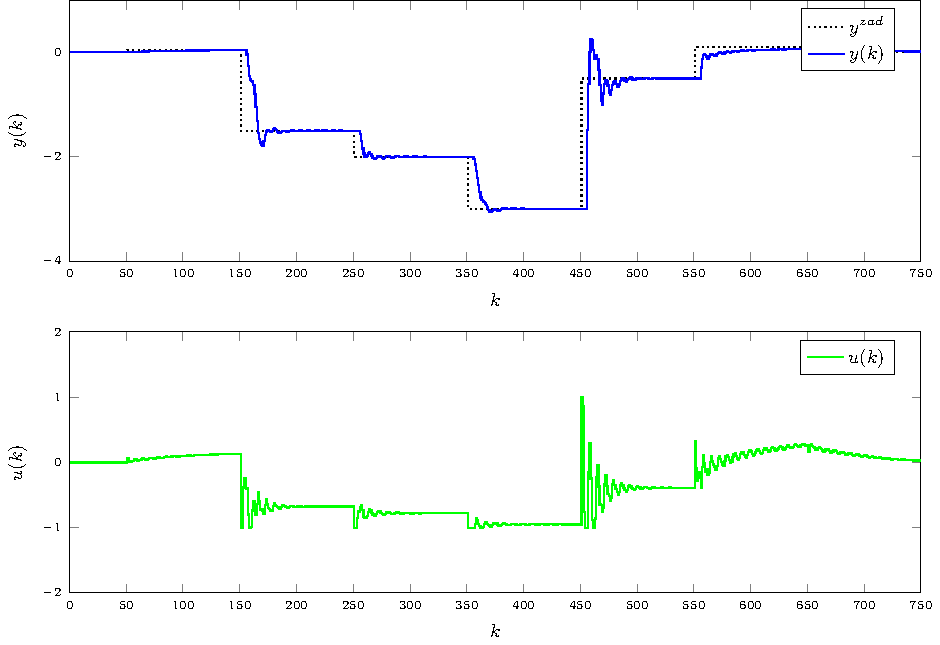
\includegraphics[width=\paperwidth]{data/exercise_7/Desired_plot_DMC_number_of_fuzzy_reg_2.pdf}}
\label{Desired_plot_DMC_number_of_fuzzy_reg_2}
\caption{eg=2}
\end{figure}
\end{center}
\newpage



\begin{table}[H]
\centering
\begin{tabular}{ | m{5em} | m{5em} |m{5em} |m{5em} |m{5em} |m{5em} | }
\hline
$D$ & $N$ & $N_u$ & $\lambda$ & $c$ & $\sigma$ \\
\hline
$\num{58}$ & $\num{16}$ & $\num{14}$ & $\num{8}$ & $\num{-2.6}$ & $\num{0.21}$ \\
\hline
$\num{49}$ & $\num{16}$ & $\num{14}$ & $\num{20}$ & $\num{-1.5}$ & $\num{0.21}$\\
\hline
$\num{39}$ & $\num{16}$ & $\num{14}$ & $\num{0.9}$ & $\num{-0.4}$ & $\num{0.21}$\\
\hline
\end{tabular}
\label{eksperyment3_DMC}
\caption{Parametry 3 rozmyte regulatory DMC}
\end{table}

\begin{center}
\begin{figure}[H]
\makebox[\textwidth]{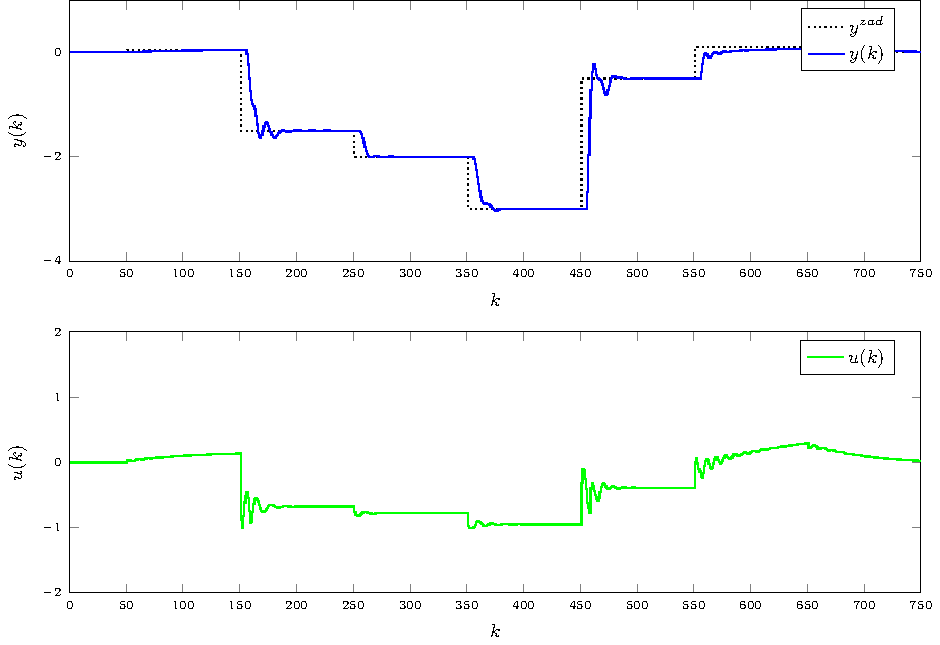
\includegraphics[width=\paperwidth]{data/exercise_7/Desired_plot_DMC_number_of_fuzzy_reg_3.pdf}}
\label{Desired_plot_DMC_number_of_fuzzy_reg_3}
\caption{eg=3}
\end{figure}
\end{center}
\newpage

\begin{table}[H]
\centering
\begin{tabular}{ | m{5em} | m{5em} |m{5em} |m{5em} |m{5em} |m{5em} | }
\hline
$D$ & $N$ & $N_u$ & $\lambda$ & $c$ & $\sigma$ \\
\hline
$\num{60}$ & $\num{15}$ & $\num{10}$ & $\num{0.1}$ & $\num{-2.8}$ & $\num{0.2}$\\
\hline
$\num{54}$ & $\num{15}$ & $\num{10}$ & $\num{30}$ & $\num{-1.98}$ & $\num{0.2}$\\
\hline
$\num{45}$ & $\num{15}$ & $\num{10}$ & $\num{15}$ & $\num{-1.2}$ & $\num{0.2}$\\
\hline
$\num{38}$ & $\num{15}$ & $\num{10}$ & $\num{0.01}$ & $\num{-0.35}$ & $\num{0.2}$\\
\hline
\end{tabular}
\label{eksperyment4_DMC}
\caption{Parametry 4 rozmyte regulatory DMC}
\end{table}

\begin{center}
\begin{figure}[H]
\makebox[\textwidth]{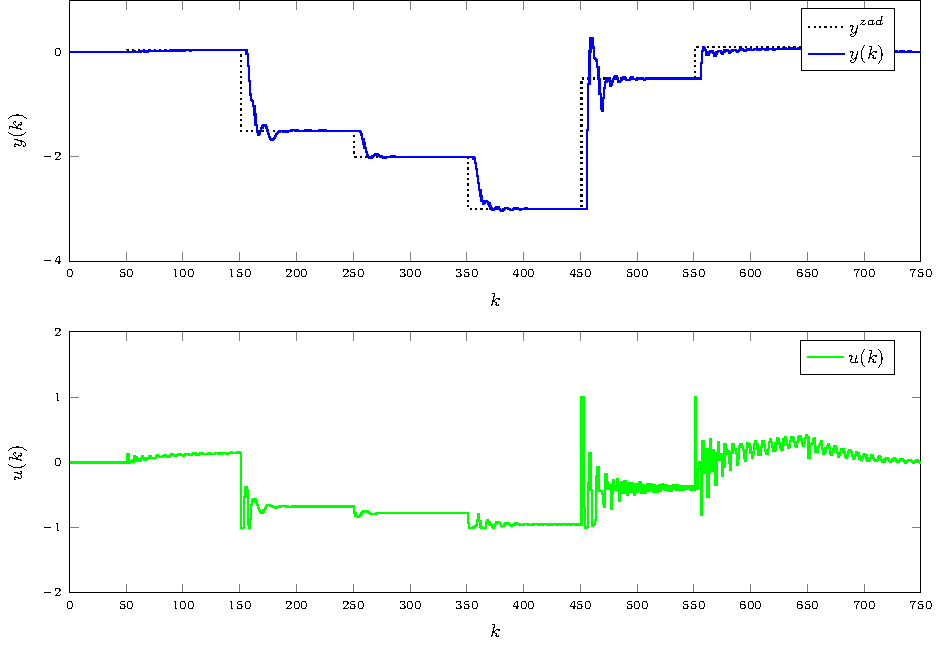
\includegraphics[width=\paperwidth]{data/exercise_7/Desired_plot_DMC_number_of_fuzzy_reg_4.pdf}}
\label{Desired_plot_DMC_number_of_fuzzy_reg_4}
\caption{eg=4}
\end{figure}
\end{center}
\newpage

\begin{table}[H]
\centering
\begin{tabular}{ | m{5em} | m{5em} |m{5em} |m{5em} |m{5em} |m{5em} | }
\hline
$D$ & $N$ & $N_u$ & $\lambda$ & $c$ & $\sigma$ \\
\hline
$\num{60}$ & $\num{14}$ & $\num{14}$ & $\num{8}$ & $\num{-2.8}$ & $\num{0.2}$\\
\hline
$\num{55}$ & $\num{14}$ & $\num{14}$ & $\num{10}$ & $\num{-2.1}$ & $\num{0.2}$\\
\hline
$\num{49}$ & $\num{14}$ & $\num{14}$ & $\num{10}$ & $\num{-1.6}$ & $\num{0.3}$\\
\hline
$\num{41}$ & $\num{14}$ & $\num{14}$ & $\num{0.6}$ & $\num{-1}$ & $\num{0.3}$\\
\hline
$\num{40}$ & $\num{14}$ & $\num{14}$ & $\num{0.2}$ & $\num{-0.5}$ & $\num{0.3}$\\
\hline
\end{tabular}
\label{eksperyment4_DMC}
\caption{Parametry 5 rozmytch regulator�w DMC}
\end{table}

\begin{center}
\begin{figure}[H]
\makebox[\textwidth]{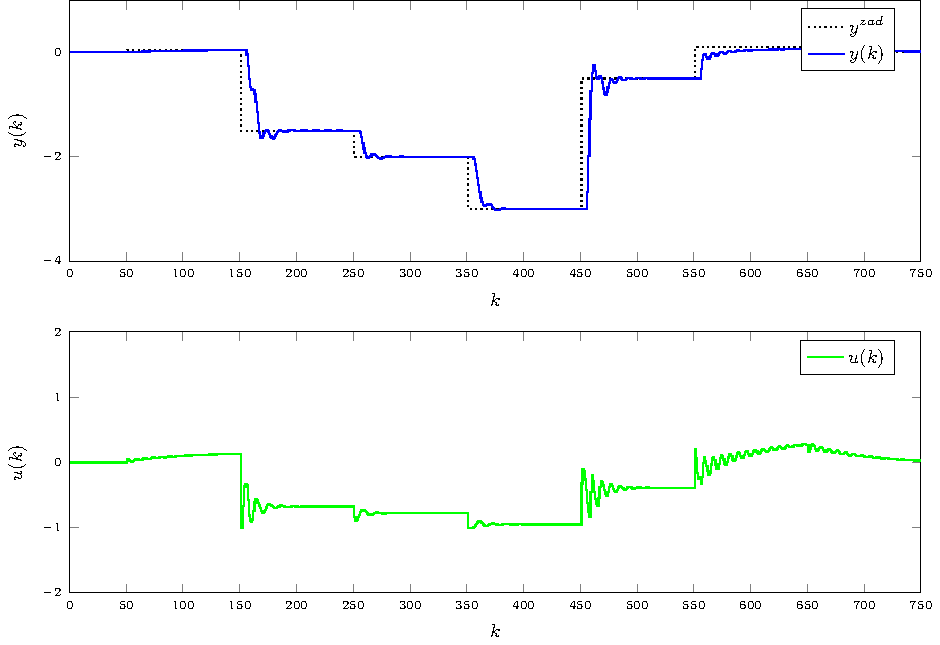
\includegraphics[width=\paperwidth]{data/exercise_7/Desired_plot_DMC_number_of_fuzzy_reg_5.pdf}}
\label{Desired_plot_DMC_number_of_fuzzy_reg_5}
\caption{eg=5}
\end{figure}
\end{center}

Jak wida� dob�r parametru lambda jest bardzo wa�na, bo pozwala w prosty spos�b poprawi� jako�� regulacji.
